\section{Interactions}

\subsection{Overview}

Figure \ref{fig:boat1} describes the system in relation to names of commands and signals of the controller and other sensor components.

\begin{figure}[!h]
	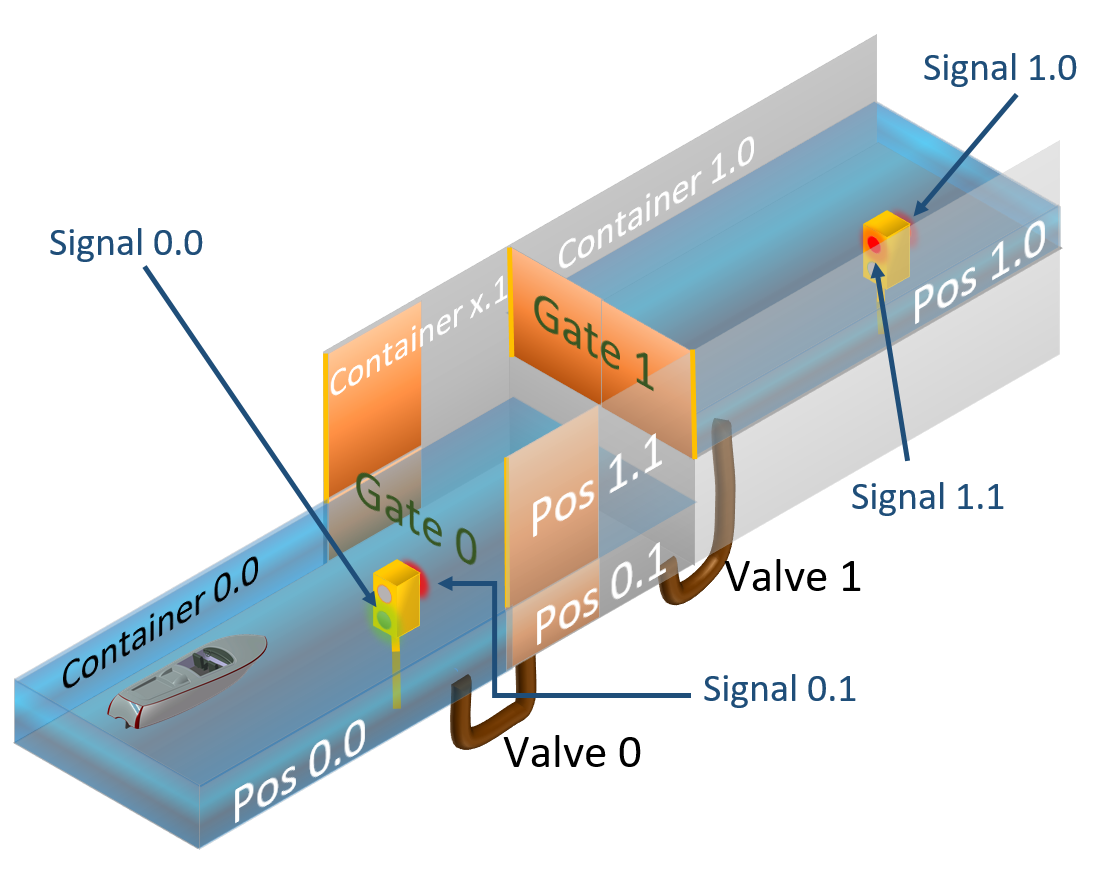
\includegraphics[width=\linewidth]{PictureName10}
	\caption{Description of the names}
	\label{fig:boat1}
\end{figure}
\pagebreak


\subsection{Commands}
\begin{table}[htbp]
	\centering
	\caption{Commands are given by the controller to the lift components and the ship operator/captain}
	\begin{tabular}{lll}
		\toprule
		\textbf{Actions} & \textbf{Description} & \textbf{Parameter} \\
		\midrule
		openGate & Open gate with the corresponding gate ID & gateID \\
		closeGate & Close gate with the corresponding gate ID & gateID \\
		openValve & Open valve with the corresponding gate ID & valveID \\
		closeValve & Close valve with the corresponding gate ID & valveID \\
		setSignalPass & Set signal to pass with the corresponding ID  & signalID \\
		setSignalHold & Set signal to hold with the corresponding ID  & signalID \\
		increaseWaterlevel & Container 1 water level increase & valveID \\
		decreaseWaterlevel & Container 1 water level decrease & valveID \\
		setIdleState & Puts the system into idle state & level \\ %level: top or bottom
		\bottomrule
		\end{tabular}%
		\label{tab:addlabel}%
		\end{table}%
		
		\subsection{Signals}
		\begin{table}[htbp]
			\centering
			\caption{These signals are generated in the lift components and sent to the controller per request (or the request is in the form of signals being sent constantly)}
			\begin{tabular}{lll}
				\toprule
				\textbf{Actions} & \textbf{Description} & \textbf{Parameter} \\
				\hline
				getGateState & Returns open (true) or closed (false) & gateID, $ \mathbb{B} $ \\
				getValveState & Returns open (true) or closed (false) & valveID, $ \mathbb{B} $ \\
				getWaterflowState & Returns on (true) or off (false) & valveID, $ \mathbb{B} $ \\
				compareWaterlevel & \parbox[t]{3in}{Compare ContainerID to Container X.1. \par Equal (true) or unequal (false)} & containerID, $ \mathbb{B} $ \\
				getSignalState & Returns pass (true) or hold (false) & signalID, $ \mathbb{B} $ \\
				getGateSensor & Returns if a ship is present (true) or not (false) & gateID, $ \mathbb{B} $ \\
				getShipPresence  & Returns if a sip is present (true) or not (false) & posID, $ \mathbb{B} $ \\
				getIdleState & Returns if the system is in idle state & level, $ \mathbb{B} $ \\
				\bottomrule
			\end{tabular}%
				\label{tab:addlabel}%
				\end{table}%
				
				
